
The site-survey stage extracts and selects a set of reference points in the indoor environment then builds up a reference point database. Instead of collecting wireless fingerprints at all coordinates, in \oursystem we just extract feature points at only a few locations for the reason that at one shooting point we are able to collect many feature points as long as no obstacle lies between us and building structure. Each reference point stored in the database is denoted as a trituple $R = (v, c, a)$ where $v$ is a vector of vision features which we refer to as the \emph{feature descriptor} in this work, $c$ represents the geographical coordinates of the reference point and $a$ denotes the visible orientation of this reference point.
% Note that the visible orientation of a reference point is affected by both the obstacles (\eg we cannot see reference points behind a wall) and the angle of viewpoint.
In this work, we leverage the state-of-the-art feature detector SURF\cite{bay2006surf}, a performant scale- and rotation-invariant interest point detector and descriptor, which is inspired by the SIFT descriptor\cite{lowe2004distinctive}, and is faster than SIFT. With this typical setting, a SURF feature descriptor can be represented as a vector with 64 dimensions.
%SIFT achieves high performance in matching to large databases. As reported in \cite{lowe2004distinctive}, there are nearly 80\% of correct matches in a database with up to 100000 key points under the condition that images have random scale and rotation changes, an affine transform of 30 degrees, and noise of 2\% added in priori.
%As the users may turn on the localization component at anywhere inside the building, the surveyed reference points should be evenly distributed all-round the indoor environment. Note that as we conduct site-survey floor by floor and users usually take picture at similar altitudes on each floor, we consider the coverage problem only on horizontal direction.
\subsection{Observations of Site Survey}

We are aiming to collect reference points associated with the building structure for the reason that these features are relatively stable.
A straight-forward solution is to take pictures at consecutive locations, as shown in Figure~\ref{fig_site-survey}(a). Let $\alpha$ denote the view angle of the camera \ie the photo can cover reference points in a range of $\alpha$ degree.
This method ensures that all reference points be recorded from one direction.
However, there is another factor which should be considered, the visible orientation of the reference points which is denoted as $\beta$. Note that the SURF features retain high matching accuracy (80\%) out to a 30 degree change in viewpoint. In other words, if the users look at the same reference point from a direction that differs from that in site-survey stage for more than 15 degree, the reference point could be unrecognizable. Therefore, in this work, we set $beta$ to 30 degree.
As shown in Figure~\ref{fig_site-survey}(a), while standing in the shadow region the user will have difficulties in identifying reference points in front.
%To address this issue, we present a simple strategy to improve the visible orientation of reference points by adding more sampling locations.

There is no need to guarantee that all reference points can be identified from all directions, thus our design goal is to approximately ensure a proper view angle in front of each reference point, which means the reference point can be recognized from the direction orthogonal to its background building structure or even tolerates small skews in view angle. As $\beta$ is usually smaller than $\alpha$, we first consider $\alpha$ as wide as $\beta$ and set the distance between two shooting points to $D\cdot \tan(\frac{\beta}{2})$ as shown in Figure~\ref{fig_site-survey}(b). $D$ denotes the distance from the shooting point to the building structures. All reference points are covered by at least two pictures taken from adjacent points. The orange range of background is sampled at both $C_1$ and $C_2$ and the visible orientation of each reference point is the superposition of the visible orientations in two samples. By geometric analysis, all reference points in the overlapping range can be recognized from the direction orthogonal to the background with an angle skew less than $\frac{\beta}{2}$ to both clockwise and anticlockwise.
In practical usage, since $\alpha$ is usually larger than $\beta$ and we can take multiple pictures in different directions in one location, we have sufficient redundancies in the quantity of reference points to ensure the accuracy of query.
\begin{figure*}[!htpb]
\centering
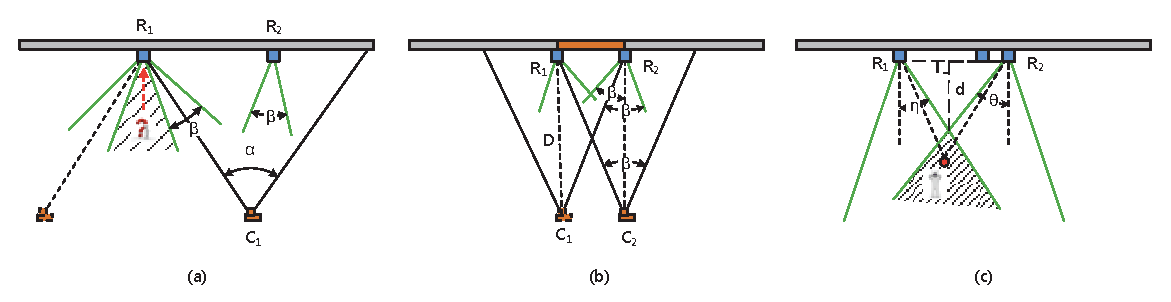
\includegraphics[width=1\linewidth,height=1.3in]{site-survey2.eps}
\caption{The observations of site-survey.}\label{fig_site-survey}
\end{figure*}
\subsection{Reference Points Geographical Coordinates Calculation}
Based on previous observations, we make a survey track according to the building structure. We annotate every shooting point in the track with its coordinates in the local coordinate system of the building. We take a pair-photo, including a left and a right photo,  at every shooting point. We use two cameras to take pair-photo, the left camera is $d_{cam}mm$ apart from the right camera.
\subsubsection{Depth Calculation}
Firstly, we will calculate the depth of feature point extracted from pair-photo using binocular ranging technique.
\begin{figure}[!hb]
\centering
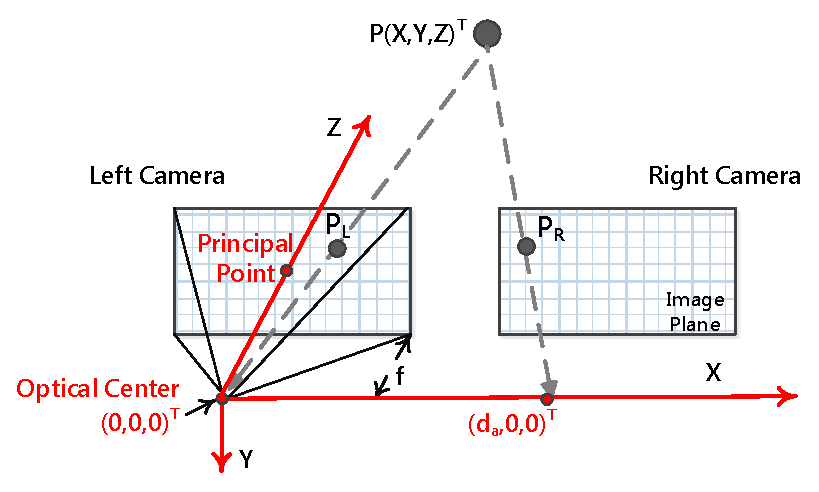
\includegraphics[ height=1.3in]{twoview2.eps}
\caption{Model of reference point's depth calculation.}\label{fig_twoview}
\end{figure}
Figure~\ref{fig_twoview} shows the geometry model of calculation for reference point's depth.
Optical center is the center of the perspective projection, the optical axis is perpendicular to the image plane piercing through the principal point on the plane.
Without loss of generality, the coordinate system is selected such that
 its origin is located at the optical center of the left camera
 and the Z-axis is collinear to the optical axis, as shown in Figure~\ref{fig_twoview}.
$P$ $(X,Y,Z)^T$ is a geographical coordinate of one feature point
 and the two corresponding projected pixels on image planes are $P_L$$(x_L,y_L)$ and $P_R$$(x_R,y_R)$, where $x_L$, $x_R$, $y_L$, $y_R$ denote pixel coordinates.
Let the principal point of left camera be $(o_x,o_y)^T$.
The projection of $P$ on the image plane of the left camera is
\begin{equation}
x_L = \frac{X\cdot f}{Z}+o_x, y_L = \frac{Y\cdot f}{Z}+o_y.
\end{equation}
Expressed in matrix:
\begin{equation}
\lambda_L \begin{pmatrix}x_L \\ y_L \\ 1 \end{pmatrix} = \begin{pmatrix}f & 0 & o_x\\0 & f & o_y\\ 0 & 0 & 1 \end{pmatrix} \begin{pmatrix}X \\ Y \\ Z\end{pmatrix}.
\end{equation}
$\lambda_L$ is a scaling factor.
Let $K=\begin{pmatrix}f & 0 & o_x\\0 & f & o_y\\ 0 & 0 & 1\end{pmatrix}$,
when the origin of the pixel coordinate system corresponds to the principal point,
 $(o_x,o_y)^T=(0,0)^T$.
The right camera is located on the $X$ axis whose optical center is $(d_{cam},0,0)$.
Because both cameras are identical, we have:
\begin{equation}
\lambda_R \begin{pmatrix}x_R \\ y_R \\ 1 \end{pmatrix} = K \begin{pmatrix}X \\ Y \\ Z\end{pmatrix} - K  \begin{pmatrix}d_{cam} \\ 0 \\ 0\end{pmatrix}.
\end{equation}
The depth $Z$ of $P$ can be expressed combining with coordinates of $P_L$ and $P_R$,
\begin{equation}
\begin{pmatrix}x_R \\ y_R \end{pmatrix} = \begin{pmatrix} {x_L-\frac{f \cdot d_{cam}}{Z}} \\ y_L \end{pmatrix},
\end{equation}
%So the depth of point $P$ is
\begin{equation}
  Z=\frac{f \cdot d_{cam}}{Disparity},
\end{equation}
where $Disparity=x_L-x_R$.
\subsubsection{Geographical Coordinates Calculation}
\begin{figure}[!hb]
\centering
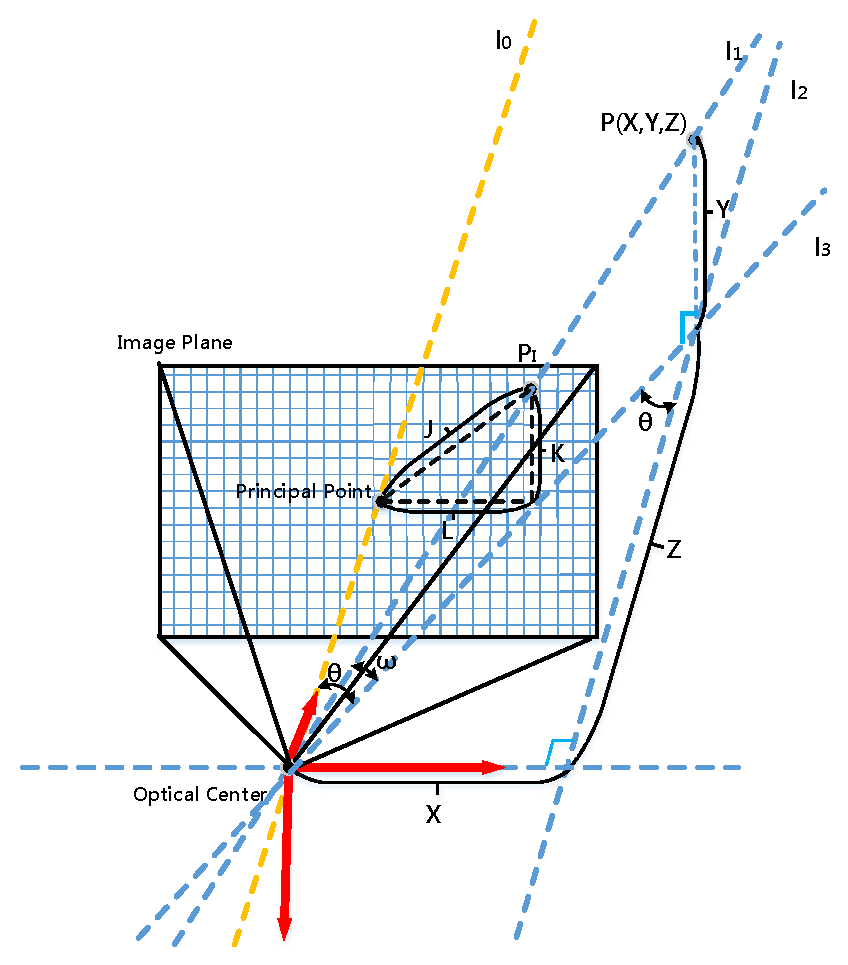
\includegraphics[width=2in, height=2in]{refgeo.eps}
\caption{Model of reference point geographical coordinates calculation.}
\label{fig_refgeo}
\end{figure}
Figure~\ref{fig_refgeo} shows the geometry model of reference point geographical coordinates calculation. As we figure out the depth Z of reference point P, we are able to calculate the coordinate $X$ and $Y$ of $P$.
\begin{equation}
    X=Z\cdot tan{\theta}
\end{equation}
where $\theta$ is the angle between $l_0$ and $l_3$, it is also as wide as the angle between $l_3$ and $l_2$. $\theta$ is proportional to $L$, which is horizontal component of pixel distance J from $P_I$ to the principal point, $P_I$ is perspective projection of point P on the image plane. The view angle $\alpha$ of camera is usually constant, so
\begin{equation}
    \theta = \frac{L\cdot \alpha}{w_{photo}}
\end{equation}
where $w_{photo}$ is the width of the photo in pixel.
Similarly, we can calculate the angle $\omega$ which is between $l_3$ and $l_2$. According to the height of optical center $h_{oc}$, we figure out
\begin{equation}
    Y=h_{oc}\pm (\sqrt{X^2+Z^2}\cdot tan{\omega} )
\end{equation}
which takes a plus sign when $P_I$ is above the principal point, minus sign when beneath.
\subsection{Reference Points Filtering}
High redundance of reference points is prone to incur high storage and search overhead. Additionally, indistinctive reference points may lead to error localization results. Therefore, it is necessary to filter the reference points to retain the most distinctive ones while ensuring the selected reference points evenly distributed in the indoor environment with desired density for localization.

To address this issue, we present an iterative filtering scheme. At the very beginning, all reference points are partitioned into different clusters according to their feature descriptors. Then reference points within each cluster are ordered by their \emph{neighbor density}, defined as the number of neighbors of one reference point with spacial distance less than $r$.

In each iteration, we select the largest cluster and check the reference point with the highest neighbor density.
Then the neighbor densities of reference points in the cluster are updated as well as their orders. If the neighbor densities of all points in a cluster are all lower than the the pre-specified threshold $D_{min}$, this cluster is marked as \emph{done} and will not be processed in the next iteration.
The above operations repeat until all clusters are marked as \emph{done}.

%Then we discuss the setting of parameters $r$, $D_{min}$.
As is shown in Figure~\ref{fig_site-survey}(c), the user can recognize both reference points $R_1$ and $R_2$ while standing in the shadow area. As is discussed in prior subsection, the angle $\eta$ and $\theta$ are within the range of $[\frac{\beta}{2}, \beta]$, thus the distance between $R_1$ and $R_2$ which is calculated as $d \cdot (\tan{\eta} + \tan{\theta})$ is within the range of $[d \cdot \tan{\beta}, 2 \cdot d \cdot \tan{\beta}]$. Here we assume that users will stand 2 meters away from the building structures at most of the times, thus $d \leq 2$. Then the distance between $R_1$ and $R_2$ should be less than $d \cdot \tan{\beta} = \frac{2}{\sqrt{3}}$. We need at least three reference points to inversely localize the user which will be discussed in following sections, so we require that at least one reference point exists between $R_1$ and $R_2$. To satisfy this condition, the distance from one reference point to its nearest neighbor should be less than $\frac{d}{2} \cdot \tan{\beta} = \frac{1}{\sqrt{3}}$. This setting is just a sufficient but not necessary condition for our localization scheme since users can change their view point to get more reference points. Then we set $r$ equal to $\frac{d}{2} \cdot \tan{\beta} = \frac{1}{\sqrt{3}}$ and $D_{min}$ equal to 1.



%\subsection{Feature skeleton construction}
%Design goal: easy site-survey, accurate feature skeleton, high quality feature filter.
%Steps:
%\begin{enumerate}
%\item Survey plan: given angle of view and floor plan how to survey.
%\item Skeleton construction: projecting features to floor plan.
%\item Feature filter: filter ''good'' features considering their quality and distribution.
%\end{enumerate}

%\subsection{Feature plane of view extraction}
%Design goal: high quality feature filter.

%Feature filter:
%\begin{enumerate}
%\item Remove noisy features from dynamic objects.
%\item Consistence with skeleton filter.
%\item Reduce communication cost by reducing the weight of centrol features. (Features near boundary are significant)
%\end{enumerate}

%\subsection{Automated Floor Plan Generation}
%\mynote{delete this section??}
%We build a coarse floor-plan from the reference points extracted in the site-survey stage.
%Reference points are grouped to different floors according to their attitudes. In each floor, the reference points are projected to plane based on their latitude and longitude. We then partition the plane into grids, the grid size is determined by the resolution of maps that we need. We regard each grid as a pixel and fill each grid with an intensity proportional to the number of reference points located in the grid.
%Thus we get an intensity image. We apply the state-of-the-art contour detection \mynote{cite a paper,figure} technique on the image to find the contour and by this way, we obtain an approximation of the floor-plan.


